% Volume II: Calculus, Analysis, and Continuous Mathematics
% Continuity note for Chapter 9.
% Previous dependencies: Chapter 3's vector geometry, norms, inner products, and angles; Chapter 4's matrix-as-linear-map viewpoint; Chapter 5's projection and fitting geometry; Chapter 7's shape-first derivative notation; Chapter 8's one-variable limits, derivatives as local linearization, integrals as accumulation, and differential-equation preview.
% New durable concepts: scalar-valued and vector-valued functions on subsets of R^n; level sets and partial dependence; partial derivatives; directional derivatives; gradients as Riesz representatives of directional change under the Euclidean inner product; Jacobians as local linear maps for vector-valued functions; chain rule for Jacobians; Hessians as matrices of second partial derivatives; curvature, definiteness, saddle points, and second-order optimality tests.
% Forward hooks: Chapter 10 reuses gradients and Hessians for Taylor approximation, optimization landscapes, manifolds, and Lagrange geometry; Chapter 11 reuses Jacobian determinants for change of variables; Chapter 12 reuses directional derivatives and operators on functions; later ML chapters reuse gradients for training, Jacobians for sensitivity and backpropagation, and Hessians/Fisher matrices for curvature and uncertainty.
% Notation commitments: x=(x_1,\ldots,x_n)^\top denotes an input vector in U\subseteq\mathbb{R}^n; scalar-valued functions are f:U\to\mathbb{R}; vector-valued functions are F:U\to\mathbb{R}^m with components F_i; gradients are column vectors \nabla f(x)\in\mathbb{R}^n; unit directions are u with \|u\|_2=1; Jacobians are J_F(x)\in\mathbb{R}^{m\times n}; Hessians are H_f(x)=\nabla^2 f(x)\in\mathbb{R}^{n\times n}; small displacements are h or \Delta x.
% Figure plan: four ImageGen raster figures under imagegen-figures/ch09-* are referenced: surface/contour views for 9.1; gradient and directional derivative geometry for 9.2; Jacobian local map geometry for 9.3; Hessian curvature and saddle/valley geometry for 9.4.
\section{Chapter 9: Multivariable Calculus}
\label{ch:multivariable-calculus}

Chapter 8 rebuilt one-variable calculus around two ideas: derivatives are local linear approximations, and integrals accumulate small pieces. Real models rarely depend on one input. A neural network loss depends on thousands or millions of weights. A firing-rate model may depend on stimulus contrast, spatial position, adaptation state, and recent spike history. A dynamical system may track many neural or artificial units at once. Multivariable calculus is the finite-dimensional calculus needed for those models.

The central problem of this chapter is: how do we describe local change when the input and output may both have many coordinates? The answer is not to memorize more derivative symbols. It is to keep the shapes clear. Scalar-valued functions have gradients and Hessians. Vector-valued functions have Jacobians. Directional derivatives ask for change along chosen directions. These objects are vectors and matrices, so the geometry of earlier chapters remains active.

\paragraph{Chapter problem.}
Given a function whose input lives in \(\mathbb{R}^n\), how do we measure sensitivity to each coordinate, to arbitrary directions, to vector outputs, and to curvature?

\paragraph{Section map.}
Section 9.1 introduces scalar-valued and vector-valued functions of many variables, domains in \(\mathbb{R}^n\), surfaces, contours, level sets, and partial derivatives. Section 9.2 defines directional derivatives and gradients, then proves the steepest-ascent interpretation. Section 9.3 treats vector-valued maps and Jacobians as local linear transformations. Section 9.4 studies Hessians, curvature, definiteness, saddle points, and second-order tests.

\subsection{9.1 Functions of many variables}

\paragraph{Motivating question.}
When a model output depends on several inputs at once, how do we represent the function and see how each variable contributes?

\paragraph{Beginner setup.}
A function of many variables accepts a vector as input. The simplest visual case is a scalar-valued function of two variables,
\[
f:\mathbb{R}^2\to\mathbb{R},
\qquad
(x,y)\mapsto f(x,y).
\]
You can picture \(f(x,y)\) as a surface whose height above the \((x,y)\)-plane is \(z=f(x,y)\). You can also picture it as a contour map: each curve contains points with the same function value.

The smallest nontrivial example is
\[
f(x,y)=x^2+2y.
\]
At the point \((1,3)\),
\[
f(1,3)=1^2+2(3)=7.
\]
If we hold \(y=3\) fixed and vary \(x\), the function becomes the one-variable slice \(g(x)=x^2+6\). If we hold \(x=1\) fixed and vary \(y\), it becomes \(h(y)=1+2y\). A multivariable function can therefore be explored by looking at slices, but the full function may contain interactions between variables that slices alone do not reveal.

This concept solves the modeling problem created by multiple explanatory variables. A loss \(L(\theta)\) depends on all parameters \(\theta_1,\ldots,\theta_n\). A neuron response model may depend on stimulus features \(s_1,\ldots,s_d\). A population state update may depend on all current activities. Writing the input as a vector keeps the object type explicit.

What to keep in mind: a point \(x\in\mathbb{R}^n\) is one input, not \(n\) unrelated inputs. Coordinates let us describe that point, but the function acts on the whole vector. Coordinate slices are useful diagnostic views; they are not the whole geometry.

\begin{figure}[htbp]
\centering
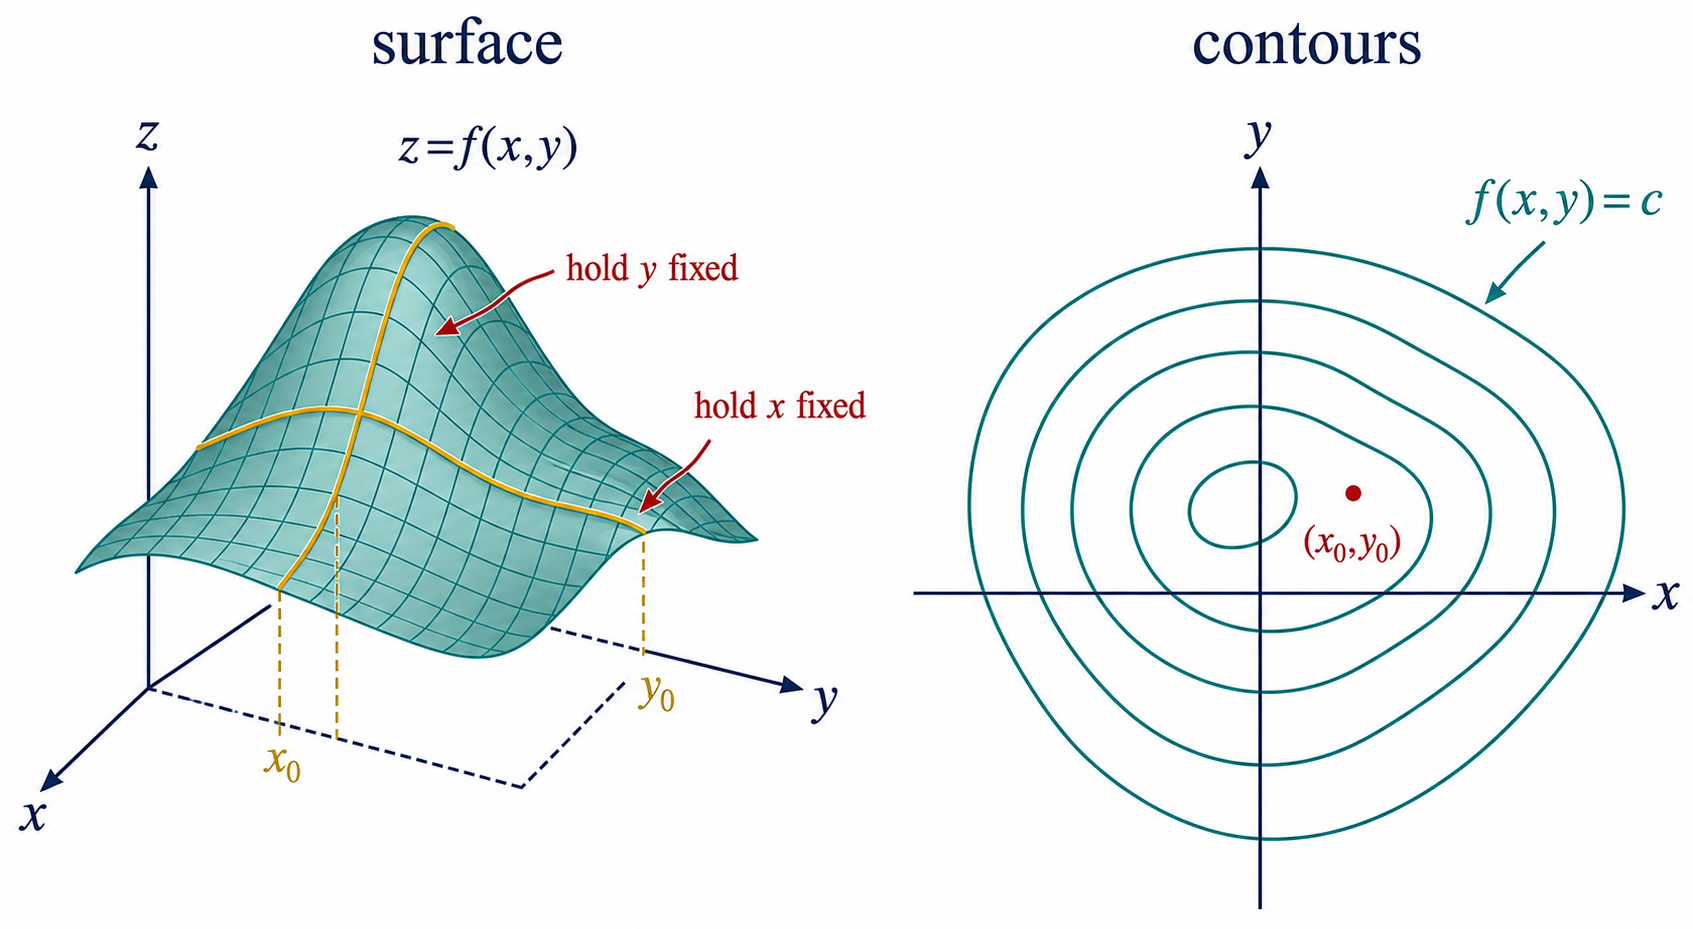
\includegraphics[width=0.95\linewidth]{imagegen-figures/ch09-functions-surface-contours.png}
\caption{A scalar-valued function of two variables can be viewed as a surface \(z=f(x,y)\) or as a contour map in the input plane. Holding one coordinate fixed gives a one-variable slice through the surface. Contours are level sets: all points on one contour share the same value of \(f\).}
\label{fig:ch09-functions-surface-contours}
\end{figure}

\paragraph{Formal setup.}
Let \(U\subseteq\mathbb{R}^n\) be a domain, usually an open set when derivatives are being taken. A scalar-valued multivariable function is
\[
f:U\to\mathbb{R},
\qquad
x=(x_1,\ldots,x_n)^\top\mapsto f(x).
\]
A vector-valued function is
\[
F:U\to\mathbb{R}^m,
\qquad
F(x)=
\begin{bmatrix}
F_1(x)\\
\vdots\\
F_m(x)
\end{bmatrix}.
\]
For a scalar-valued function \(f\), a \emph{level set} at level \(c\in\mathbb{R}\) is
\[
\{x\in U:f(x)=c\}.
\]
In \(\mathbb{R}^2\), level sets are often contour curves. In \(\mathbb{R}^3\), they are often surfaces.

The partial derivative with respect to coordinate \(x_i\) at \(a\in U\) is the one-variable derivative obtained by changing only the \(i\)th coordinate:
\[
\frac{\partial f}{\partial x_i}(a)
=
\lim_{t\to 0}
\frac{f(a+t e_i)-f(a)}{t},
\]
provided the limit exists and \(a+t e_i\in U\) for small \(t\). Here \(e_i\) is the \(i\)th standard basis vector. This equation belongs to multivariable functions because it defines coordinate-wise sensitivity while keeping the other coordinates fixed.

\paragraph{Core intuition.}
Figure~\ref{fig:ch09-functions-surface-contours} shows two complementary views of the same scalar function. The surface view answers, "What height does the function assign to this input point?" The contour view answers, "Which input changes keep the output unchanged?" A contour map is often more useful for optimization because it lets us draw directions of change in the input space.

Partial derivatives are slopes of coordinate slices. If \(f(x,y)\) is a landscape, then \(\partial f/\partial x\) is the slope you feel when you walk east-west while holding north-south position fixed. The derivative \(\partial f/\partial y\) is the slope you feel when you walk north-south while holding east-west position fixed. If the function has an interaction term such as \(xy\), the \(x\)-slope may depend on the current value of \(y\). That is why multivariable calculus is not just many separate copies of one-variable calculus.

A common beginner misconception is that knowing all coordinate slices away from a point automatically explains the whole surface. Slices help, but the function may bend differently in diagonal directions. Another misconception is treating the domain as always all of \(\mathbb{R}^n\). Many important functions have constraints: probabilities live on a simplex, covariance matrices must be positive semidefinite, and normalized activity vectors may lie on a sphere. Constraints change which directions are allowed.

This section builds on Chapter 2's domain/codomain discipline and Chapter 3's vector geometry. It prepares gradients, Jacobians, Hessians, constrained surfaces, and vector fields. In later chapters, \(f\) may be a loss function, a density, an energy, or a scalar summary of neural activity.

\paragraph{Main derivation: partial derivatives as coordinate-slice derivatives.}
Let \(f:\mathbb{R}^2\to\mathbb{R}\) be
\[
f(x,y)=x^2+3xy+y^2.
\]
At a point \((a,b)\), the partial derivative with respect to \(x\) is computed by changing \(x\) and holding \(y=b\) fixed:
\[
\frac{\partial f}{\partial x}(a,b)
=\lim_{t\to 0}\frac{f(a+t,b)-f(a,b)}{t}.
\]
Expand the numerator:
\[
f(a+t,b)=(a+t)^2+3(a+t)b+b^2
=a^2+2at+t^2+3ab+3tb+b^2.
\]
Subtract \(f(a,b)=a^2+3ab+b^2\):
\[
f(a+t,b)-f(a,b)=2at+t^2+3tb.
\]
Divide by \(t\):
\[
\frac{f(a+t,b)-f(a,b)}{t}=2a+t+3b.
\]
Letting \(t\to0\) gives
\[
\frac{\partial f}{\partial x}(a,b)=2a+3b.
\]
Similarly,
\[
\frac{\partial f}{\partial y}(a,b)=3a+2b.
\]
The algebra teaches the mechanism: a partial derivative is an ordinary derivative along a coordinate line, but the other coordinates remain present as fixed values.

\paragraph{Worked examples.}
\emph{Small symbolic example.} For
\[
f(x,y)=x^2+3xy+y^2,
\]
the value at \((1,2)\) is
\[
f(1,2)=1+6+4=11.
\]
The partial derivatives are
\[
\frac{\partial f}{\partial x}=2x+3y,
\qquad
\frac{\partial f}{\partial y}=3x+2y.
\]
At \((1,2)\),
\[
\frac{\partial f}{\partial x}(1,2)=8,
\qquad
\frac{\partial f}{\partial y}(1,2)=7.
\]
Near \((1,2)\), changing \(x\) by \(0.01\) while holding \(y\) fixed changes \(f\) by about \(0.08\); changing \(y\) by \(0.01\) while holding \(x\) fixed changes \(f\) by about \(0.07\).

\emph{ML/neuroscience example.} Let
\[
L(w_1,w_2)=\frac{1}{2}\left((w_1+2w_2)-3\right)^2
\]
be the squared error of a one-neuron linear model on one training example with input features \(1\) and \(2\), target \(3\), and weights \(w_1,w_2\). This is a scalar-valued function \(L:\mathbb{R}^2\to\mathbb{R}\). Its value is a loss height over weight space. The contour map shows weight pairs with equal error. The partial derivative with respect to \(w_1\) asks how loss changes if only the first synaptic weight changes; the partial derivative with respect to \(w_2\) asks the same for the second weight.

\paragraph{ML/DL/neuroscience connections.}
In machine learning, a training loss is a scalar-valued function on parameter space: \(L:\mathbb{R}^n\to\mathbb{R}\). The input vector \(x\) in the calculus notation becomes the parameter vector \(\theta\), and the output \(L(\theta)\) is a scalar objective. In deep learning, an activation map may be vector-valued because many units output many coordinates. In neuroscience, a firing-rate field \(r(s_1,s_2)\) may map a two-dimensional stimulus or spatial location to a scalar rate, while a population response map \(R(s)\in\mathbb{R}^m\) maps a stimulus to \(m\) neuron responses. Level sets become iso-response curves: stimulus changes along one level set preserve the modeled response.

\paragraph{Exercises.}
\begin{enumerate}[label=\textbf{9.1.\arabic*.}, leftmargin=*]
\item \textbf{Mechanical.} For \(f(x,y,z)=x^2+yz+3z\), compute \(f(1,2,-1)\), \(\partial f/\partial x\), \(\partial f/\partial y\), and \(\partial f/\partial z\).
\item \textbf{Proof or derivation.} Starting from the limit definition of \(\partial f/\partial x\), derive \(\partial f/\partial x=2x+y^2\) for \(f(x,y)=x^2+xy^2\).
\item \textbf{Numerical/computational.} Approximate \(\partial f/\partial y(1,2)\) for \(f(x,y)=\sin(xy)\) using the finite difference \(\bigl(f(1,2+h)-f(1,2)\bigr)/h\) with \(h=10^{-2}\) and \(h=10^{-4}\). Compare with the exact value.
\item \textbf{Interpretation.} For a loss \(L(w_1,w_2)\), what does the level set \(\{(w_1,w_2):L(w_1,w_2)=1\}\) mean in model space?
\item \textbf{Debug the misconception.} A student says, "If \(\partial f/\partial x=0\), the function is locally constant." Explain why this is false for multivariable functions, and give a simple example.
\end{enumerate}

\subsection{9.2 Gradients and directional derivatives}

\paragraph{Motivating question.}
If a scalar function has many input directions, which direction increases it fastest, and how much does it change along a chosen direction?

\paragraph{Beginner setup.}
A partial derivative measures change in one coordinate direction. A \emph{directional derivative} measures change along any chosen direction. If \(u\in\mathbb{R}^n\) is a unit vector, then the directional derivative of \(f\) at \(a\) in direction \(u\) is
\[
D_u f(a)=\lim_{t\to0}\frac{f(a+t u)-f(a)}{t}.
\]
The \emph{gradient} collects all first partial derivatives into one vector:
\[
\nabla f(a)=
\begin{bmatrix}
\frac{\partial f}{\partial x_1}(a)\\
\vdots\\
\frac{\partial f}{\partial x_n}(a)
\end{bmatrix}.
\]
For differentiable functions under the Euclidean inner product,
\[
D_u f(a)=\nabla f(a)^\top u.
\]

The smallest nontrivial example is \(f(x,y)=x^2+y^2\). At \(a=(1,2)^\top\),
\[
\nabla f(a)=
\begin{bmatrix}2\\4\end{bmatrix}.
\]
In the unit direction \(u=(1,0)^\top\), the directional derivative is \(2\). In the unit direction \(v=(0,1)^\top\), it is \(4\). In the diagonal unit direction \(q=(1,1)^\top/\sqrt{2}\), it is \(6/\sqrt{2}\). Different directions expose different slopes through the same point.

What to keep in mind: the gradient is not merely a list of partial derivatives. It is the vector that converts a direction into a first-order rate of change by a dot product. Its direction is steepest ascent, and its length is the largest directional derivative among unit directions.

\begin{figure}[htbp]
\centering
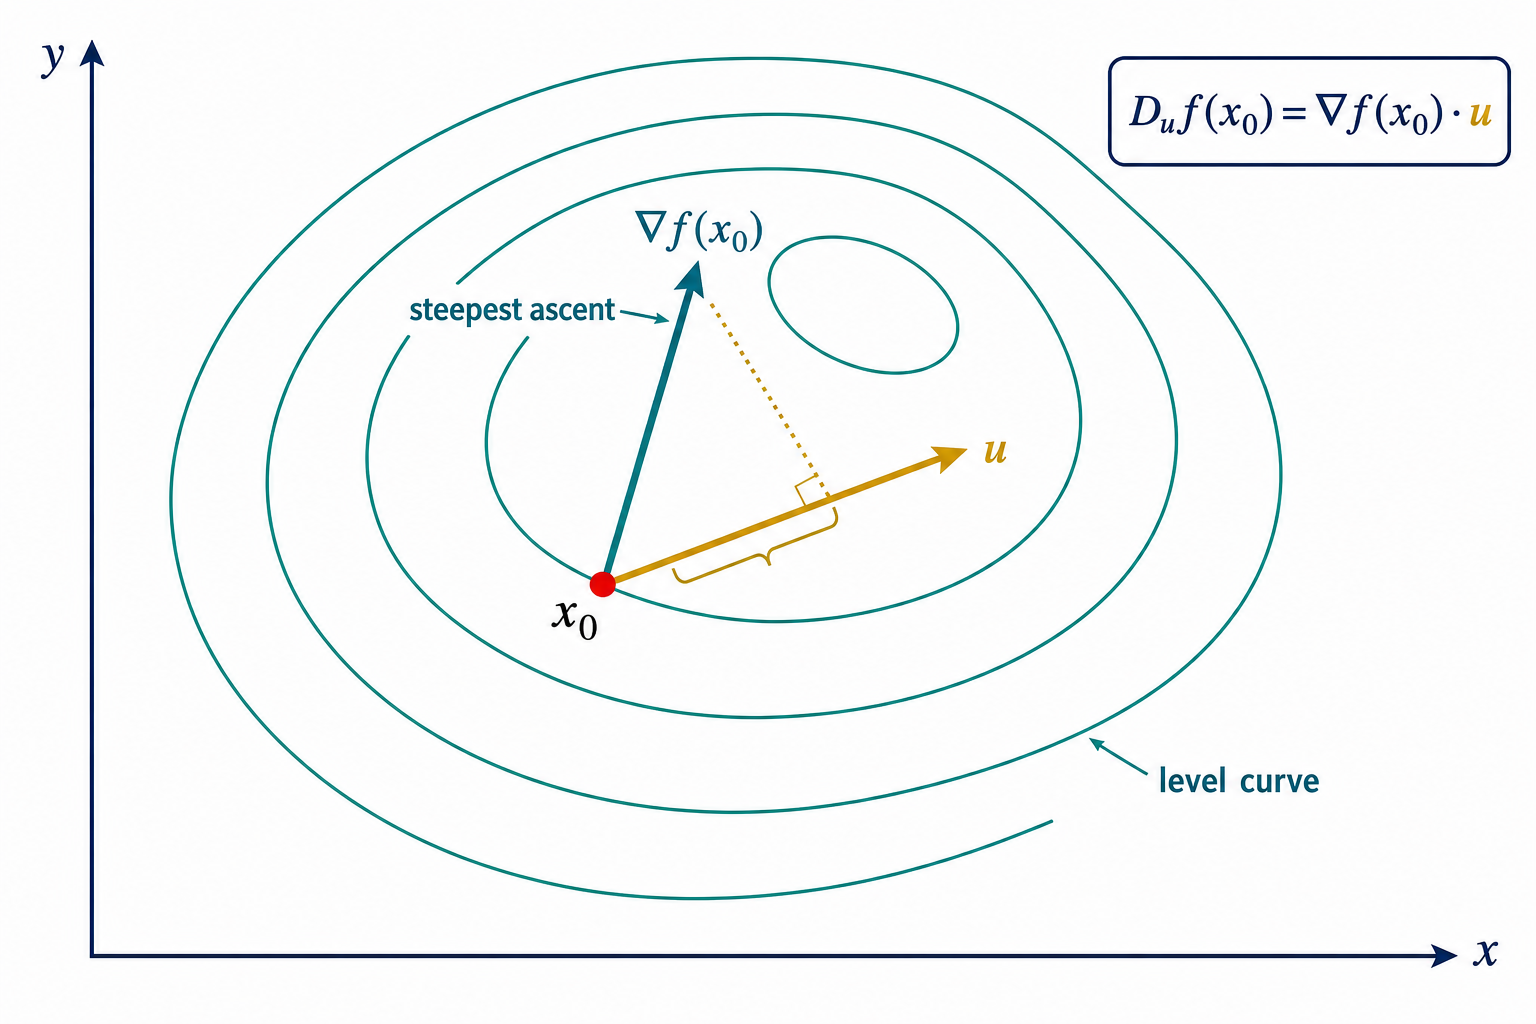
\includegraphics[width=0.94\linewidth]{imagegen-figures/ch09-gradient-directional-derivative.png}
\caption{The gradient \(\nabla f(x_0)\) is perpendicular to the level curve through \(x_0\) and points toward steepest first-order increase. The directional derivative \(D_u f(x_0)\) is the dot product \(\nabla f(x_0)^\top u\), so it is the component of the gradient in the chosen unit direction \(u\).}
\label{fig:ch09-gradient-directional-derivative}
\end{figure}

\paragraph{Formal setup.}
Let \(U\subseteq\mathbb{R}^n\), let \(f:U\to\mathbb{R}\), and let \(a\in U\). A direction \(u\in\mathbb{R}^n\) is usually normalized so \(\|u\|_2=1\); otherwise the derivative scales with the length of the direction vector. The directional derivative is
\[
D_u f(a)=\lim_{t\to0}\frac{f(a+t u)-f(a)}{t},
\]
when the limit exists. If \(f\) is differentiable at \(a\), then there is a linear map \(Df(a):\mathbb{R}^n\to\mathbb{R}\) such that
\[
f(a+h)=f(a)+Df(a)[h]+o(\|h\|_2).
\]
In Euclidean coordinates, this linear map is represented by the gradient:
\[
Df(a)[h]=\nabla f(a)^\top h.
\]
Therefore the central equation of this section is
\[
D_u f(a)=\nabla f(a)^\top u.
\]
The domain of \(\nabla f\) is the set of points where \(f\) is differentiable; its value lies in \(\mathbb{R}^n\), the same vector space as the input directions.

\paragraph{Core intuition.}
Figure~\ref{fig:ch09-gradient-directional-derivative} shows why gradients and contours fit together. Moving along a level curve keeps \(f\) unchanged, so the directional derivative tangent to the level curve is zero. The gradient is perpendicular to that tangent because its dot product with every first-order no-change direction is zero. Moving in the gradient direction crosses contours as quickly as possible.

The dot product formula also explains signs. If \(u\) points mostly with the gradient, \(D_u f(a)>0\). If \(u\) is perpendicular to the gradient, \(D_u f(a)=0\). If \(u\) points against the gradient, \(D_u f(a)<0\). This is a local, first-order statement. A large step can leave the local region where the derivative is a good guide.

Two misconceptions are especially common. First, a zero gradient does not always mean a minimum. It means no first-order direction of change. The point might be a maximum, saddle, or flat point. Hessians in Section 9.4 help distinguish these cases. Second, the phrase "steepest" depends on the chosen norm and inner product. In this course, unless stated otherwise, steepest means steepest under the Euclidean norm.

This section connects directly back to inner products from Chapter 3. The gradient is the vector that represents the derivative linear functional through the Euclidean dot product. It connects forward to gradient descent, backpropagation, constrained optimization, and vector fields. A vector field assigns a vector to each point; a gradient field is the special vector field \(x\mapsto\nabla f(x)\) built from a scalar potential \(f\).

\paragraph{Main theorem: gradient as steepest ascent.}
Suppose \(f:U\to\mathbb{R}\) is differentiable at \(a\), and \(\nabla f(a)\neq0\). Among all unit directions \(u\), the directional derivative \(D_u f(a)\) is maximized by
\[
u_\star=\frac{\nabla f(a)}{\|\nabla f(a)\|_2},
\]
and the maximum value is
\[
\|\nabla f(a)\|_2.
\]

\emph{Proof sketch.} For any unit vector \(u\),
\[
D_u f(a)=\nabla f(a)^\top u.
\]
By Cauchy-Schwarz,
\[
\nabla f(a)^\top u\leq \|\nabla f(a)\|_2\|u\|_2=\|\nabla f(a)\|_2.
\]
Equality in Cauchy-Schwarz occurs when \(u\) points in the same direction as \(\nabla f(a)\). Since \(u\) must have unit length, the equality direction is
\[
u_\star=\frac{\nabla f(a)}{\|\nabla f(a)\|_2}.
\]
Thus the gradient direction gives steepest first-order ascent, and the negative gradient direction gives steepest first-order descent.

\paragraph{Worked examples.}
\emph{Small numerical example.} Let
\[
f(x,y)=x^2+xy+2y^2.
\]
Then
\[
\nabla f(x,y)=
\begin{bmatrix}
2x+y\\
x+4y
\end{bmatrix}.
\]
At \(a=(1,1)^\top\),
\[
\nabla f(a)=
\begin{bmatrix}3\\5\end{bmatrix}.
\]
For the unit direction \(u=(1,2)^\top/\sqrt{5}\),
\[
D_u f(a)
=
\begin{bmatrix}3&5\end{bmatrix}
\frac{1}{\sqrt{5}}
\begin{bmatrix}1\\2\end{bmatrix}
=\frac{13}{\sqrt{5}}.
\]
The steepest-ascent rate is
\[
\|\nabla f(a)\|_2=\sqrt{3^2+5^2}=\sqrt{34},
\]
which is larger than \(13/\sqrt{5}\), as the theorem predicts.

\emph{ML/neuroscience example.} Let \(L(\theta)\) be a training loss for a model with parameter vector \(\theta\in\mathbb{R}^n\). The gradient \(\nabla L(\theta)\) is the vector of first-order sensitivities of the loss to every parameter. Gradient descent updates
\[
\theta_{k+1}=\theta_k-\eta\nabla L(\theta_k),
\]
where \(\eta>0\) is a step size. The negative gradient is the steepest local descent direction under the Euclidean norm, but the step size still matters. If \(\eta\) is too large, the update can overshoot the region where the first-order approximation is accurate. In neuroscience, if \(f(s)\) is a firing-rate surface over stimulus features \(s\), then \(\nabla f(s)\) points in the stimulus direction that most rapidly increases the modeled firing rate.

\paragraph{ML/DL/neuroscience connections.}
In deep learning, backpropagation computes gradients of a scalar loss with respect to many parameter arrays. The mathematical object \(\nabla L(\theta)\) becomes the collection of all parameter sensitivities, flattened or shape-organized by layer. In adversarial examples, the gradient with respect to the input points toward small input perturbations that most increase loss. In neural coding, gradients of tuning curves identify stimulus directions with high response sensitivity. In dynamical systems, a vector field \(\dot{x}=v(x)\) assigns a direction of motion to each state; if \(v(x)=-\nabla E(x)\), trajectories descend an energy function \(E\).

\paragraph{Exercises.}
\begin{enumerate}[label=\textbf{9.2.\arabic*.}, leftmargin=*]
\item \textbf{Mechanical.} Compute \(\nabla f(x,y)\) for \(f(x,y)=3x^2-2xy+y^2\). Then compute \(D_u f(1,-1)\) for \(u=(1,1)^\top/\sqrt{2}\).
\item \textbf{Proof or derivation.} Use Cauchy-Schwarz to prove that the negative gradient direction gives the smallest directional derivative among all unit directions.
\item \textbf{Numerical/computational.} For \(f(x,y)=x^2+4y^2\), start at \((2,1)\) and take one gradient-descent step with \(\eta=0.1\). Compute the new point and compare \(f\) before and after the step.
\item \textbf{Interpretation.} On a contour map of a loss function, why is the gradient perpendicular to the contour through the current parameter vector?
\item \textbf{Debug the misconception.} A student says, "If \(\nabla f(a)=0\), then \(a\) is definitely the best point." Explain what the gradient does and does not tell us, and name two other possibilities.
\end{enumerate}

\subsection{9.3 Jacobians and vector-valued functions}

\paragraph{Motivating question.}
When a function has many outputs, what matrix describes how a small input change affects all output coordinates at once?

\paragraph{Beginner setup.}
A vector-valued function maps one vector to another:
\[
F:\mathbb{R}^n\to\mathbb{R}^m.
\]
Instead of one scalar output, it has \(m\) component functions:
\[
F(x)=
\begin{bmatrix}
F_1(x)\\
\vdots\\
F_m(x)
\end{bmatrix}.
\]
The \emph{Jacobian} is the matrix of all first partial derivatives:
\[
J_F(x)=
\begin{bmatrix}
\frac{\partial F_1}{\partial x_1}(x)&\cdots&\frac{\partial F_1}{\partial x_n}(x)\\
\vdots&\ddots&\vdots\\
\frac{\partial F_m}{\partial x_1}(x)&\cdots&\frac{\partial F_m}{\partial x_n}(x)
\end{bmatrix}
\in\mathbb{R}^{m\times n}.
\]

The smallest useful example is
\[
F(x,y)=
\begin{bmatrix}
x^2+y\\
xy
\end{bmatrix}.
\]
This map takes a two-dimensional input to a two-dimensional output. Its Jacobian is
\[
J_F(x,y)=
\begin{bmatrix}
2x&1\\
y&x
\end{bmatrix}.
\]
At \((1,2)\), this becomes
\[
J_F(1,2)=
\begin{bmatrix}
2&1\\
2&1
\end{bmatrix}.
\]
If the input changes by \(\Delta x=(0.01,-0.02)^\top\), the output change is approximately
\[
J_F(1,2)\Delta x
=
\begin{bmatrix}
2&1\\
2&1
\end{bmatrix}
\begin{bmatrix}
0.01\\
-0.02
\end{bmatrix}
=
\begin{bmatrix}
0\\
0
\end{bmatrix}.
\]
To first order, this particular displacement moves along a local no-change direction for both outputs.

What to keep in mind: the Jacobian is not a new kind of object unrelated to matrices. It is the matrix of the best local linear approximation to a vector-valued function.

\begin{figure}[htbp]
\centering
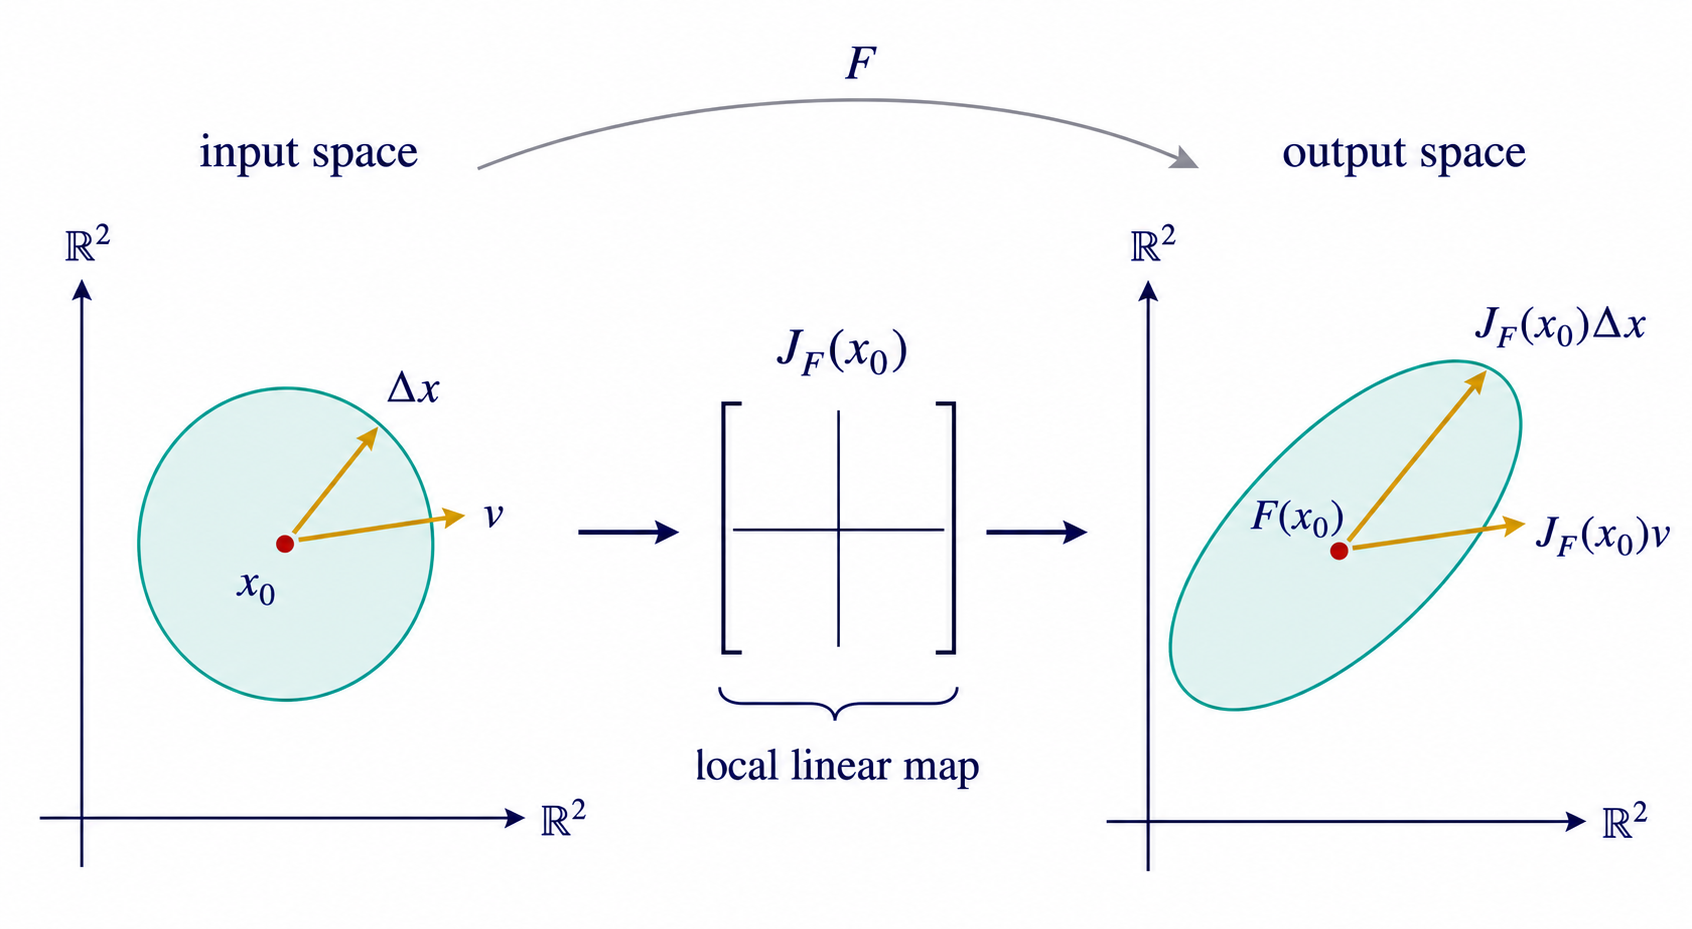
\includegraphics[width=0.96\linewidth]{imagegen-figures/ch09-jacobian-local-map.png}
\caption{The Jacobian \(J_F(x_0)\) is the local linear map that sends small input displacements near \(x_0\) to first-order output displacements near \(F(x_0)\). A small circle of possible input perturbations becomes an ellipse or parallelogram under the linearized map.}
\label{fig:ch09-jacobian-local-map}
\end{figure}

\paragraph{Formal setup.}
Let \(U\subseteq\mathbb{R}^n\), and let \(F:U\to\mathbb{R}^m\) have component functions \(F_1,\ldots,F_m\). If every component is differentiable at \(a\), the derivative of \(F\) at \(a\) is a linear map
\[
DF(a):\mathbb{R}^n\to\mathbb{R}^m.
\]
In standard coordinates, this linear map is represented by the Jacobian matrix \(J_F(a)\in\mathbb{R}^{m\times n}\). The central local approximation is
\[
F(a+h)\approx F(a)+J_F(a)h,
\qquad h\in\mathbb{R}^n\text{ small}.
\]
The shape matters: \(J_F(a)\) has \(m\) rows and \(n\) columns because it maps an \(n\)-dimensional input displacement \(h\) to an \(m\)-dimensional output displacement.

For a scalar-valued function \(f:U\to\mathbb{R}\), the Jacobian is a \(1\times n\) row matrix,
\[
J_f(a)=
\begin{bmatrix}
\frac{\partial f}{\partial x_1}(a)&\cdots&\frac{\partial f}{\partial x_n}(a)
\end{bmatrix},
\]
while the gradient is usually stored as the corresponding \(n\times1\) column vector. This row-versus-column convention is a source of shape errors, so always check what the derivative must multiply.

\paragraph{Core intuition.}
Figure~\ref{fig:ch09-jacobian-local-map} extends Chapter 4's matrix-as-map picture. A nonlinear function may bend large regions, but near a point it can often be replaced by a linear map. The Jacobian is that local matrix. If you draw a small ball around the input point, the Jacobian sends it to the linearized shape in output space. Stretching, compression, rotation, and shear are all possible because the Jacobian is a matrix.

Rows and columns have different meanings. The \(i\)th row is the gradient of output component \(F_i\) written as a row; it tells how the \(i\)th output changes with input directions. The \(j\)th column tells how all output coordinates change when input coordinate \(x_j\) changes. When \(F\) is a neural network layer or a population response map, rows correspond to output units and columns correspond to input features or upstream units.

Common misconceptions come from scalar habits. First, a vector-valued function does not have one gradient; each scalar component has a gradient, and the Jacobian stacks them. Second, the Jacobian is local. A large input change may not be well predicted by one Jacobian if the map curves strongly. Third, the determinant of a Jacobian only makes sense when \(m=n\); rectangular Jacobians still describe sensitivity but not signed volume scaling by a determinant.

This section prepares the chain rule used in neural networks, normalizing flows, dynamical systems, and change of variables. It also gives the local view of vector fields: a vector field \(V:\mathbb{R}^n\to\mathbb{R}^n\) assigns a velocity to every state, and \(J_V(x)\) describes how nearby velocities differ.

\paragraph{Main theorem: Jacobian chain rule.}
Let
\[
G:\mathbb{R}^n\to\mathbb{R}^m,
\qquad
F:\mathbb{R}^m\to\mathbb{R}^p
\]
be differentiable at the relevant points. For the composition \(H=F\circ G:\mathbb{R}^n\to\mathbb{R}^p\),
\[
J_H(a)=J_F(G(a))\,J_G(a).
\]

\emph{Proof sketch.} The local approximations are
\[
G(a+h)=G(a)+J_G(a)h+\text{small error},
\]
and, for a small output displacement \(k\),
\[
F(G(a)+k)=F(G(a))+J_F(G(a))k+\text{small error}.
\]
Use \(k=J_G(a)h+\text{small error}\). Then
\[
F(G(a+h))
\approx F(G(a))+J_F(G(a))J_G(a)h.
\]
Since the derivative is the linear map that gives the first-order output change as a function of \(h\), the Jacobian of the composition is the matrix product \(J_F(G(a))J_G(a)\). The order matches function composition: \(G\) acts on the input first, and \(F\)'s derivative acts afterward.

\paragraph{Worked examples.}
\emph{Small numerical example.} Let
\[
G(x,y)=
\begin{bmatrix}
x+y\\
xy
\end{bmatrix},
\qquad
F(u,v)=
\begin{bmatrix}
u^2\\
u+v
\end{bmatrix}.
\]
Then
\[
J_G(x,y)=
\begin{bmatrix}
1&1\\
y&x
\end{bmatrix},
\qquad
J_F(u,v)=
\begin{bmatrix}
2u&0\\
1&1
\end{bmatrix}.
\]
At \(a=(1,2)\), \(G(a)=(3,2)^\top\), so
\[
J_F(G(a))=
\begin{bmatrix}
6&0\\
1&1
\end{bmatrix},
\qquad
J_G(a)=
\begin{bmatrix}
1&1\\
2&1
\end{bmatrix}.
\]
The chain rule gives
\[
J_{F\circ G}(a)
=
\begin{bmatrix}
6&0\\
1&1
\end{bmatrix}
\begin{bmatrix}
1&1\\
2&1
\end{bmatrix}
=
\begin{bmatrix}
6&6\\
3&2
\end{bmatrix}.
\]

\emph{ML/neuroscience example.} Consider a layer
\[
z=\sigma(Wx+b),
\]
where \(x\in\mathbb{R}^n\), \(W\in\mathbb{R}^{m\times n}\), \(b\in\mathbb{R}^m\), and \(\sigma\) is applied componentwise. The Jacobian with respect to \(x\) is
\[
J_z(x)=D_\sigma(Wx+b)W,
\]
where \(D_\sigma(Wx+b)\) is the diagonal matrix with entries \(\sigma'((Wx+b)_i)\). This matrix maps a small input perturbation to the first-order perturbation of layer activations. In a neural population model \(R(s)\in\mathbb{R}^m\), the Jacobian \(J_R(s)\) maps a small stimulus displacement to predicted changes in all \(m\) neuron responses.

\paragraph{ML/DL/neuroscience connections.}
Backpropagation is repeated application of the Jacobian chain rule, organized so that full Jacobian matrices usually do not have to be materialized. Saliency methods use input-output Jacobians to identify which input features most affect a score. Recurrent neural networks and biological dynamical systems use Jacobians of state-update maps to study local stability: if nearby perturbations are expanded, trajectories separate; if they are contracted, trajectories converge. In normalizing flows, square Jacobians and their determinants measure local volume changes, a topic returned to in Chapter 11.

\paragraph{Exercises.}
\begin{enumerate}[label=\textbf{9.3.\arabic*.}, leftmargin=*]
\item \textbf{Mechanical.} Compute the Jacobian of \(F(x,y,z)=(x+y,\ yz,\ x^2+z)^\top\). State its shape.
\item \textbf{Proof or derivation.} For \(F:\mathbb{R}^n\to\mathbb{R}^m\), explain why the \(i\)th row of \(J_F(a)\) is the gradient of the scalar component \(F_i\) written as a row.
\item \textbf{Numerical/computational.} For \(F(x,y)=(x^2+y,\ xy)^\top\), compute \(J_F(1,2)\Delta x\) for \(\Delta x=(0.01,0.03)^\top\). Then compute the exact difference \(F((1,2)^\top+\Delta x)-F(1,2)\) and compare.
\item \textbf{Interpretation.} In a layer \(z=\sigma(Wx+b)\), what do the rows and columns of the Jacobian with respect to \(x\) represent?
\item \textbf{Debug the misconception.} A student says, "The Jacobian is the gradient of a vector-valued function." Rewrite that statement correctly using component functions and matrix shape.
\end{enumerate}

\subsection{9.4 Hessians and curvature}

\paragraph{Motivating question.}
After the gradient tells us the first-order direction of change, how do we describe bending, curvature, minima, maxima, and saddle points?

\paragraph{Beginner setup.}
For a scalar-valued function \(f:\mathbb{R}^n\to\mathbb{R}\), the \emph{Hessian} is the matrix of second partial derivatives:
\[
H_f(x)=\nabla^2 f(x)=
\begin{bmatrix}
\frac{\partial^2 f}{\partial x_1\partial x_1}(x)&\cdots&\frac{\partial^2 f}{\partial x_1\partial x_n}(x)\\
\vdots&\ddots&\vdots\\
\frac{\partial^2 f}{\partial x_n\partial x_1}(x)&\cdots&\frac{\partial^2 f}{\partial x_n\partial x_n}(x)
\end{bmatrix}.
\]
The gradient tells local slope. The Hessian tells how the gradient changes as the input moves.

The smallest nontrivial example is
\[
f(x,y)=x^2+3y^2.
\]
Then
\[
\nabla f(x,y)=
\begin{bmatrix}
2x\\
6y
\end{bmatrix},
\qquad
H_f(x,y)=
\begin{bmatrix}
2&0\\
0&6
\end{bmatrix}.
\]
The curvature in the \(y\)-direction is larger than the curvature in the \(x\)-direction. Contours are ellipses rather than circles because the function bends more sharply along one axis.

What to keep in mind: the Hessian is local curvature information. It does not describe the entire landscape unless the function is exactly quadratic. But near a point, it is the matrix that controls the second-order correction to the linear approximation.

\begin{figure}[htbp]
\centering
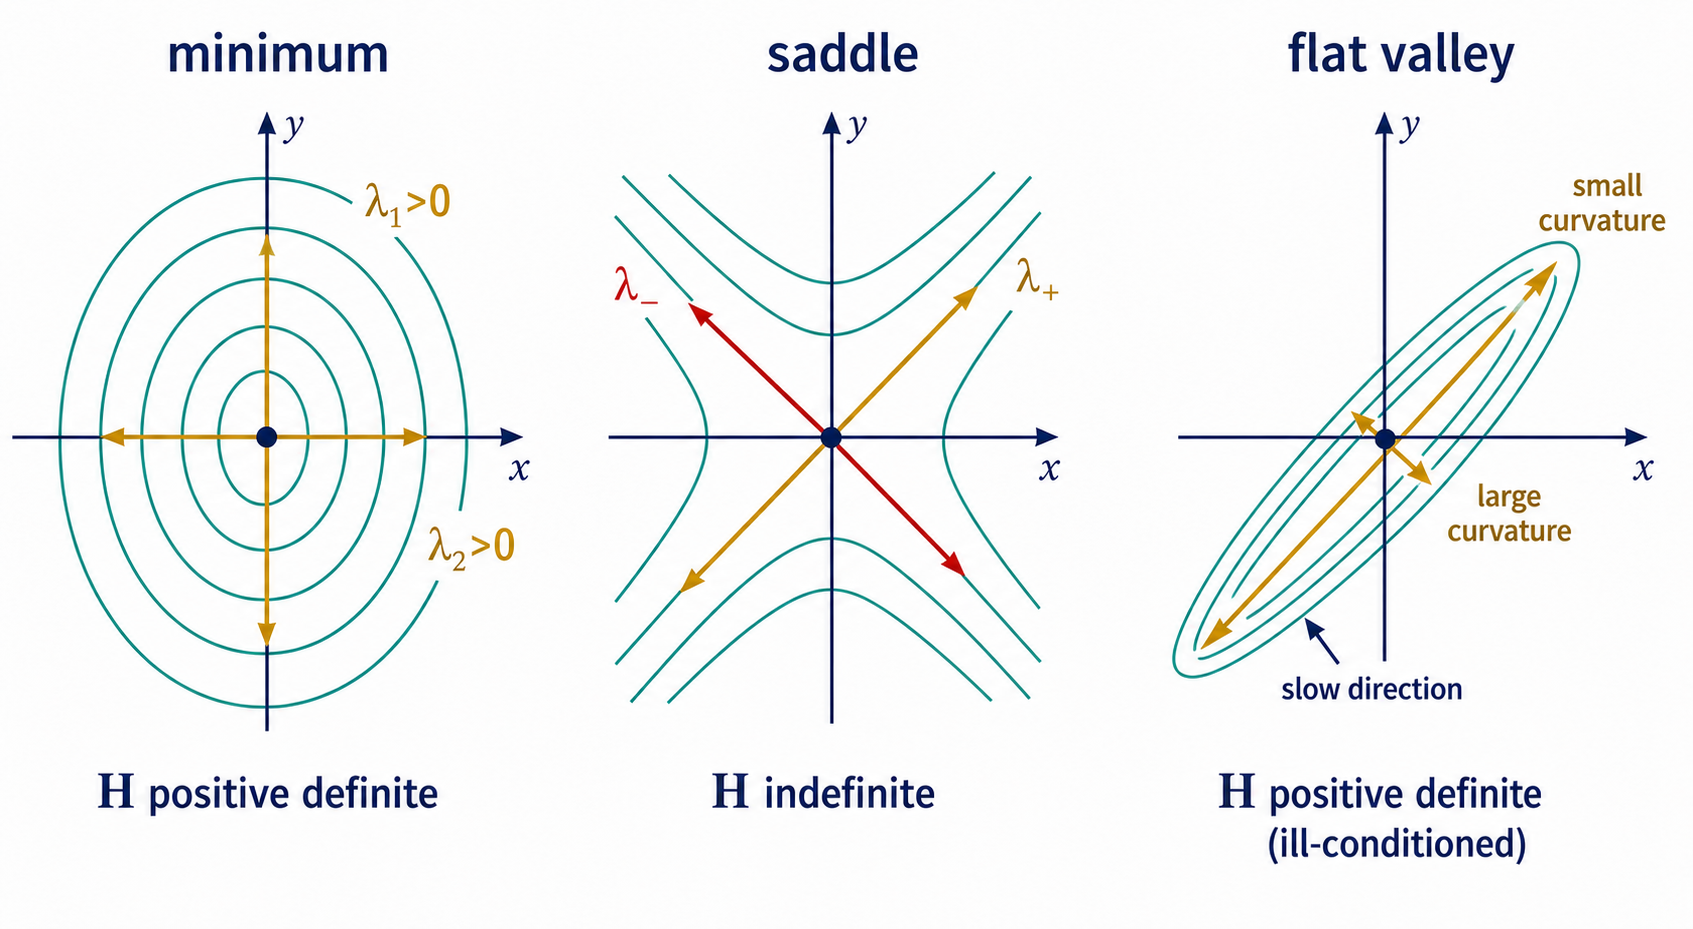
\includegraphics[width=0.96\linewidth]{imagegen-figures/ch09-hessian-curvature.png}
\caption{Hessians classify local quadratic geometry. Positive eigenvalues in all directions give a local minimum shape. Mixed signs give a saddle: some directions curve up and others curve down. Very different positive eigenvalues produce a narrow valley, which makes first-order optimization slow along the small-curvature direction.}
\label{fig:ch09-hessian-curvature}
\end{figure}

\paragraph{Formal setup.}
Let \(U\subseteq\mathbb{R}^n\), and let \(f:U\to\mathbb{R}\) have continuous second partial derivatives near \(a\). The Hessian \(H_f(a)\in\mathbb{R}^{n\times n}\) has entries
\[
\left[H_f(a)\right]_{ij}
=
\frac{\partial^2 f}{\partial x_i\partial x_j}(a).
\]
Under the continuity assumption on second partial derivatives, mixed partials agree:
\[
\frac{\partial^2 f}{\partial x_i\partial x_j}(a)
=
\frac{\partial^2 f}{\partial x_j\partial x_i}(a),
\]
so \(H_f(a)\) is symmetric.

The central second-order local model is
\[
f(a+h)\approx f(a)+\nabla f(a)^\top h+\frac{1}{2}h^\top H_f(a)h.
\]
The quadratic form \(h^\top H_f(a)h\) measures curvature in the direction \(h\). For a unit vector \(u\), the second directional derivative is
\[
\frac{d^2}{dt^2}f(a+t u)\bigg|_{t=0}=u^\top H_f(a)u.
\]

\paragraph{Core intuition.}
Figure~\ref{fig:ch09-hessian-curvature} shows three local contour geometries. At a minimum with positive curvature in all directions, contours close around the point. At a saddle, one direction curves upward while another curves downward. In a flat valley, curvature is positive but very uneven: optimization can make quick progress across the valley and slow progress along it.

Because Hessians are symmetric under standard smoothness assumptions, their eigenvectors form orthogonal curvature directions. Eigenvalues tell the curvature along those directions. Positive eigenvalues mean the function bends upward; negative eigenvalues mean it bends downward; eigenvalues near zero mean the function is locally flat in that direction.

The most common misconception is that a zero gradient proves a minimum. A zero gradient says the linear term in the local approximation is gone. The quadratic term may still be positive, negative, or mixed. Another misconception is that curvature must be visible from a one-dimensional slice. A saddle can look like a minimum in one slice and a maximum in another, so directions matter.

This section connects backward to quadratic forms in Chapter 6 and forward to Taylor approximation in Chapter 10. It also prepares optimization, uncertainty approximations, Newton methods, natural gradients, Fisher information, and local stability analysis in dynamical systems.

\paragraph{Main theorem: second-order test for critical points.}
Let \(f:U\to\mathbb{R}\) have continuous second partial derivatives near \(a\), and suppose \(\nabla f(a)=0\).
\begin{itemize}[leftmargin=*]
\item If \(H_f(a)\) is positive definite, then \(a\) is a strict local minimum.
\item If \(H_f(a)\) is negative definite, then \(a\) is a strict local maximum.
\item If \(H_f(a)\) has both positive and negative eigenvalues, then \(a\) is a saddle point.
\end{itemize}
If \(H_f(a)\) has zero eigenvalues and is only positive semidefinite or negative semidefinite, this basic test is inconclusive; higher-order terms or additional analysis are needed.

\emph{Proof sketch.} With \(\nabla f(a)=0\), the second-order model becomes
\[
f(a+h)-f(a)\approx \frac{1}{2}h^\top H_f(a)h.
\]
If \(H_f(a)\) is positive definite, then \(h^\top H_f(a)h>0\) for every nonzero \(h\), so nearby nonzero displacements increase \(f\) to second order. With sufficient smoothness, the small neglected terms cannot overturn this sign for small enough \(h\), so \(a\) is a strict local minimum. The negative definite case is the same with signs reversed.

If the Hessian has both positive and negative eigenvalues, choose unit eigenvectors \(v_+\) and \(v_-\) with eigenvalues \(\lambda_+>0\) and \(\lambda_-<0\). Along \(h=t v_+\),
\[
\frac{1}{2}h^\top H_f(a)h=\frac{1}{2}t^2\lambda_+>0.
\]
Along \(h=t v_-\),
\[
\frac{1}{2}h^\top H_f(a)h=\frac{1}{2}t^2\lambda_-<0.
\]
The function increases in one nearby direction and decreases in another, which is the local geometry of a saddle.

\paragraph{Worked examples.}
\emph{Small numerical example.} Consider
\[
f(x,y)=x^2-y^2.
\]
Then
\[
\nabla f(x,y)=
\begin{bmatrix}
2x\\
-2y
\end{bmatrix},
\qquad
H_f(x,y)=
\begin{bmatrix}
2&0\\
0&-2
\end{bmatrix}.
\]
At \((0,0)\), the gradient is zero. The Hessian has one positive and one negative eigenvalue, so \((0,0)\) is a saddle. Along the \(x\)-axis, \(f(t,0)=t^2>0\). Along the \(y\)-axis, \(f(0,t)=-t^2<0\).

For comparison, if
\[
g(x,y)=x^2+3y^2,
\]
then
\[
H_g=
\begin{bmatrix}
2&0\\
0&6
\end{bmatrix}
\]
is positive definite, and \((0,0)\) is a strict local minimum. The larger eigenvalue \(6\) means sharper curvature in the \(y\)-direction.

\emph{ML/neuroscience example.} Near a trained parameter vector \(\hat{\theta}\), a loss can be approximated by
\[
L(\hat{\theta}+h)\approx L(\hat{\theta})+\frac{1}{2}h^\top H_L(\hat{\theta})h
\]
when \(\nabla L(\hat{\theta})\approx0\). Large positive Hessian eigenvalues indicate directions where the loss rises quickly if parameters move. Small eigenvalues indicate flat directions where many parameter settings have similar training loss. In recurrent neural dynamics \(\dot{x}=F(x)\), the Jacobian describes first-order state sensitivity; when the dynamics descend an energy \(E\), the Hessian of \(E\) describes curvature of the energy landscape around equilibria.

\paragraph{ML/DL/neuroscience connections.}
Second-order optimization methods use Hessian information to rescale gradient steps. Newton's method for minimizing a smooth function uses
\[
x_{k+1}=x_k-H_f(x_k)^{-1}\nabla f(x_k),
\]
when the Hessian is invertible and the local quadratic approximation is trustworthy. In deep learning, full Hessians are usually too large to store, but Hessian-vector products and curvature approximations help analyze sharpness, flatness, and training stability. In probabilistic modeling, the negative Hessian of a log-likelihood near its maximum gives a local Gaussian uncertainty approximation. In neuroscience, energy-landscape and attractor models use curvature to distinguish stable basins, unstable directions, and slow modes.

\paragraph{Exercises.}
\begin{enumerate}[label=\textbf{9.4.\arabic*.}, leftmargin=*]
\item \textbf{Mechanical.} Compute the gradient and Hessian of \(f(x,y)=2x^2+xy+y^2\). Is the Hessian positive definite? Use eigenvalues or the \(2\times2\) determinant test.
\item \textbf{Proof or derivation.} For a symmetric Hessian \(H\), show that the curvature of the quadratic form \(q(h)=\frac{1}{2}h^\top Hh\) along a unit eigenvector \(v\) with eigenvalue \(\lambda\) is \(\lambda\).
\item \textbf{Numerical/computational.} For \(f(x,y)=x^2+10y^2\), take one gradient-descent step from \((1,1)\) with \(\eta=0.05\). Then explain why the \(y\)-coordinate changes much more than the \(x\)-coordinate.
\item \textbf{Interpretation.} A trained model has many Hessian eigenvalues close to zero near a minimum. What does this suggest about nearby parameter perturbations and loss sensitivity?
\item \textbf{Debug the misconception.} A student says, "Since \(\nabla f(0,0)=0\) for \(f(x,y)=x^2-y^2\), the origin is a minimum." Use the Hessian or directional slices to correct the claim.
\end{enumerate}

\paragraph{Closing bridge.}
This chapter turned local change into concrete finite-dimensional objects: gradients for scalar sensitivity, Jacobians for vector-valued local maps, and Hessians for curvature. Chapter 10 uses these same objects to build Taylor approximations and local geometry systematically. The first-order term will become the tangent-plane model, the second-order term will become the local quadratic model, and constraints will lead to manifolds and Lagrange geometry. Later, probability and inference will reuse the same Jacobian and Hessian ideas for transformed densities, likelihood curvature, and information geometry.

\clearpage
